\chapter{Results}

\section{Target archived}

The goal to archive includes logical and technical targets both. 
The improvements reached by thesis development are the following one

\newline
The main target to reach is to improve Value Chain \footnote{This process includes the following phases: design and development of the product,
raw materials management, production, shipping, selling and final use} value of the overall system.
\newline
The goal could be splitted inside \textbf{Technical Goal} and \textbf{Logical Goal}.

\begin{outline}
    \1 \textbf{Technical Goal}
    \2 \textbf{Crosschain Interaction}: Integrate in the same application both permissioned and permissionless
    Blockchain networks. The integration was done application side, there's some API endpoints that start
    transactions in both networks, one over fabric network and the other one over ethereum.
    \2 \textbf{Traceability}: This goal is archived implementing smart contracts, hyperledger fabric side
    that track all the clothes box and store the entire transactions passed over the system. 
    
    \1 \textbf{Logical Goal}
    \2 \textbf{Supply Chain}: The target is to simplify the supply chain process, all the steps inside the chain
    is handled as transactions, stored over the ledger and updating world state and smart contract data. 
    \2 \textbf{Susteinability}: The entire process is aims to support susteinability. Using treacebility feature
    it's possible to follow the lifetime of the clothes until they finish to Producer, that perform the 
    material recycling in order to produce new upcycled clothes.   
    \2 \textbf{Counterfeiting}: Assign a UID to each clothes produced it's possible to fight the Counterfeiting
    implementing new feature such us the clothes registrations, we're going to have a secure register contining
    all the clothes.
\end{outline}

\section{Use Case Test}

\subsection{Use Case 1 - Unit Test 1}

\subsubsection{Send Box and Evaluation}

Performing the Test over the Use Case 1 about the send box and evaluation processes. The following
figures show the results over the call of the related methods and how application works. 

The \textbf{Figure \ref{fig:user-send-box}} show the log when User Perform the \textit{Send Box} action.

\begin{figure}[h!]
	\centering
    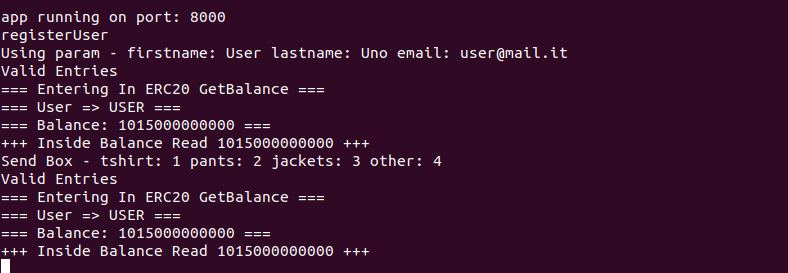
\includegraphics[totalheight=4cm]{img/test/test1/user-send-box.png}
	\caption{User Send Box}
	\label{fig:user-send-box}
\end{figure}

Once the Box Request was successfully send, the smart contract is invoked and the transaction is 
performed. Admin could see the pending box request to be evaluated. Then the Reclothes Admin UI side
insert the value amount of the tokens and start the evaluation process.
\newline
The \textbf{Figures \ref{fig:init-tx-reclothes-user}} and \textbf{\ref{fig:tx-reclothes-user}} 
show the Fabric Transaction performed then the inizialization of the Ethereum Transaction
and at the end once the eth transaction was performed the etherscan link, associated to the 
related TransactionHash, that allow to see the transaction history and infos.

\begin{figure}[h!]
	\centering
    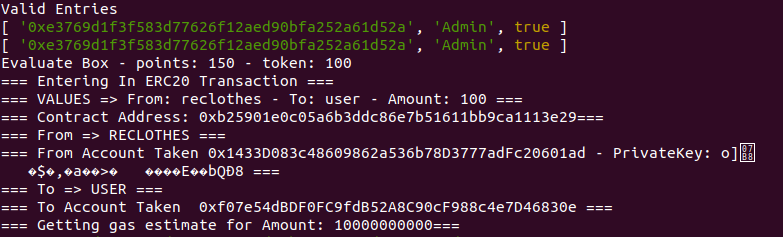
\includegraphics[totalheight=4cm]{img/test/test1/init-tx-RU.png}
	\caption{Init Transaction from Reclothes to User}
	\label{fig:init-tx-reclothes-user}
\end{figure}

\begin{figure}[h!]
	\centering
    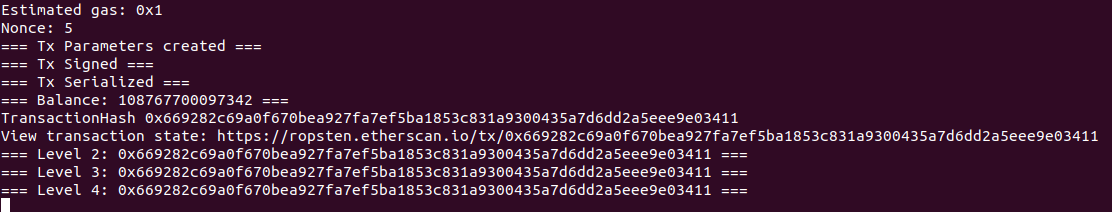
\includegraphics[totalheight=3cm]{img/test/test1/performed-tx-RU.png}
	\caption{Init Transaction from Reclothes to User}
	\label{fig:tx-reclothes-user}
\end{figure}

The Figure \ref{fig:fabric-tx} and Figure \ref{fig:eth-tx} shows the proof of the transacactions succed. 
The first Figure show the User page that could visualize the history of transactions done and all
related requests. The second one show the etherscan page with all the informations about ethereum
transaction, in this case from Reclothes eth Account to User Account. 

\begin{figure}[h!]
	\centering
    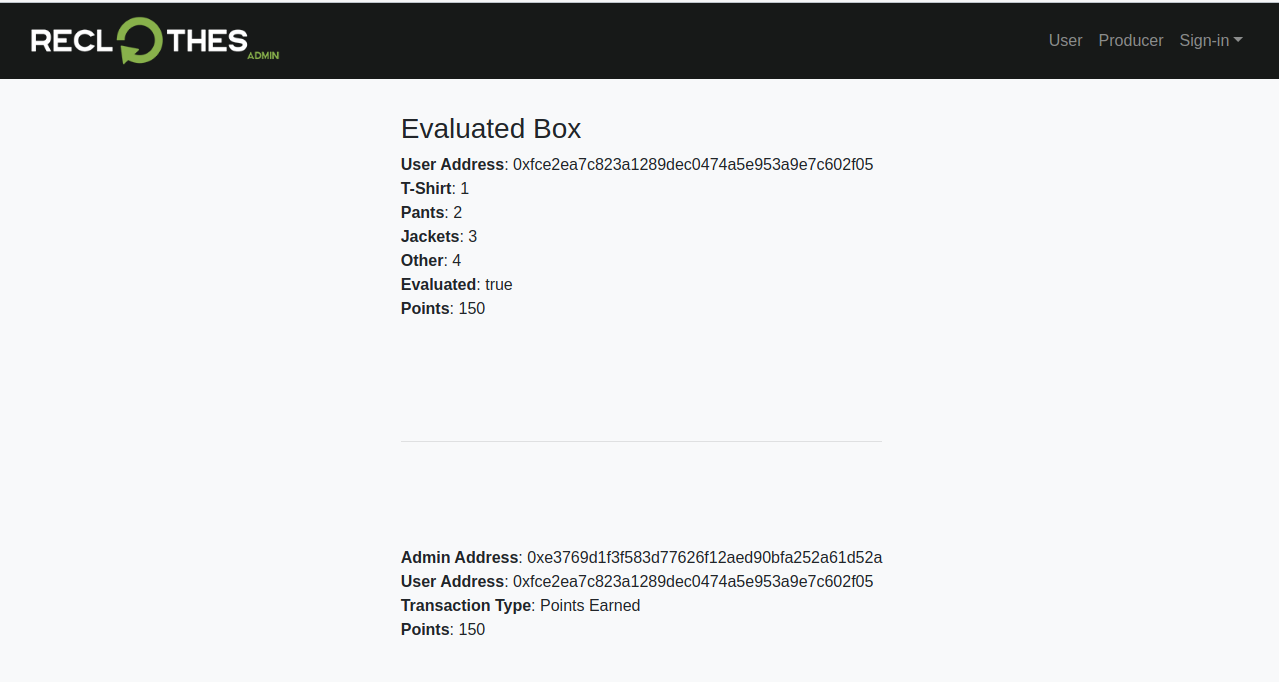
\includegraphics[totalheight=7cm]{img/test/test1/fabrix-tx.png}
	\caption{Fabric transaction history}
	\label{fig:fabric-tx}
\end{figure}

\begin{figure}[h!]
	\centering
    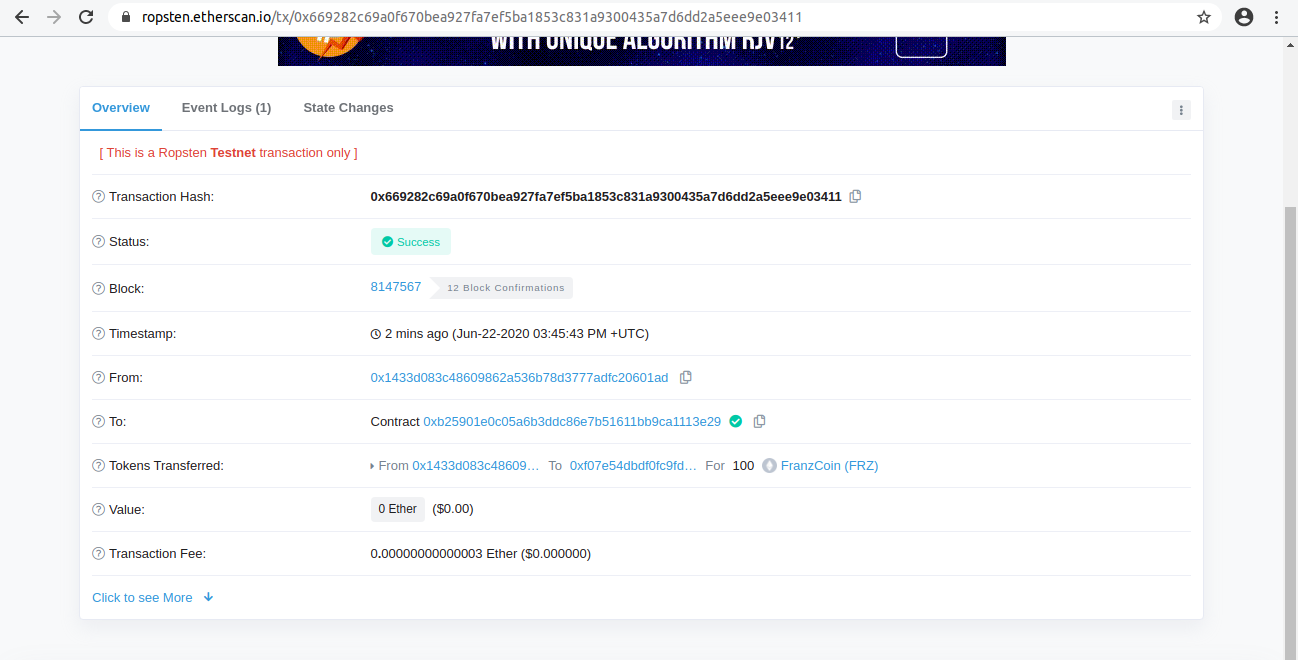
\includegraphics[totalheight=7cm]{img/test/test1/etherscan.png}
	\caption{Ethereum transaction over etherscan}
	\label{fig:eth-tx}
\end{figure}

\subsection{Use Case 1 - Unit Test 2}

\subsubsection{Purchase Item}

The \textbf{Figures \ref{fig:tx-user-reclothes}} shows the Purchase process. As figure shows
there's first of all the fabric transaction and then the eth transactions, after performed all
the previous check start the transaction from User account to Reclothes account. Once the 
transaction is performed the method print the etherscan link to monitor the transaction and
all related infos. 

\begin{figure}[h!]
	\centering
    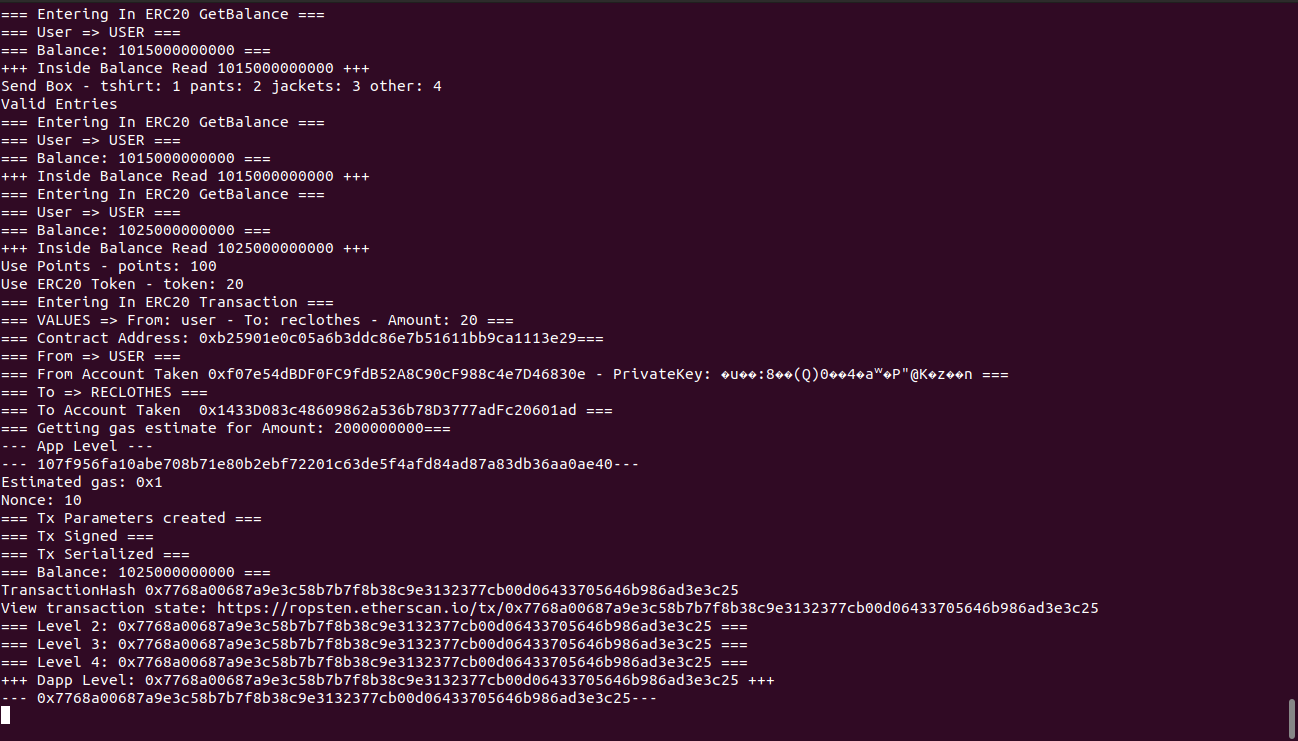
\includegraphics[totalheight=7cm]{img/test/test2/tx-user-reclothes.png}
	\caption{Transaction from User to Reclothes}
	\label{fig:tx-user-reclothes}
\end{figure}


\subsection{Use Case 2 - Unit Test 1}

To test the Use Case 2 we're going to track the behaviour of two process:

\begin{outline}
    \1 \textbf{Send Old Material and Evaluation}: The Admin for Producer send a box within old materials
    to be recycled. Once the box arrived to Producer, than it's going to be evaluated and there's a 
    Regeneration Credits transaction from Producer to AdminP.

    \1 \textbf{Purchase Upcycled Material}: The Admin for Producer spend the earned Regeneration Credits
    to purchase by Producer recycled materials. The purchase options right now are three:
    \2 \textbf{Small Box}: for 50 regeneration credits for 5 upcycled items.
    \2 \textbf{Medium Box}: for 150 regeneration credits for 15 upcycled items.
    \2 \textbf{Big Box}: for 200 regeneration credits for 40 upcycled items.
\end{outline}

\subsubsection{Send Old Material and Evaluation}

The \textbf{Figures \ref{fig:send-old-clothes}} show the log of the send old clothes process.
In that case we're going to send a box with inside: 
\begin{outline}
    \1 \textbf{t-shirt}: 10
    \1 \textbf{pants}: 20
    \1 \textbf{jacket}: 10
    \1 \textbf{other}: 10
\end{outline}

\begin{figure}[h!]
	\centering
    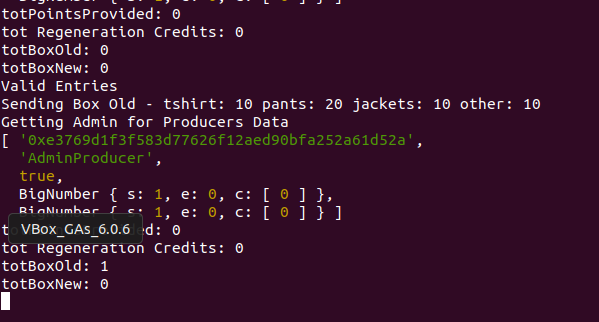
\includegraphics[totalheight=6cm]{img/test/usecase2/0-send-old-clothes.png}
	\caption{Admin Send old clothes}
	\label{fig:send-old-clothes}
\end{figure}

Once the box is sent than start the evaluation process. The Producer evaluate materials received
and issue Regeneration Credits amount that Admins could spend when need, to purchase
recycled items. The \textbf{Figure \ref{fig:1-box-tobe-evaluate.png}} shows the page used
to perform evaluation Process by Producer. In that case we set a Regeneration Credits amount
of 1200, \textbf{Figure \ref{fig:evaluation-old-clothes}} shows the output of the evaluation process.
\\
Once the evaluation process is archived and the Regeneration Credits is section
from Producer to Admin, \textbf{Figure \ref{fig:evaluation-old-clothes}} show the info update
of the Admin for Producer.

\begin{figure}[h!]
	\centering
    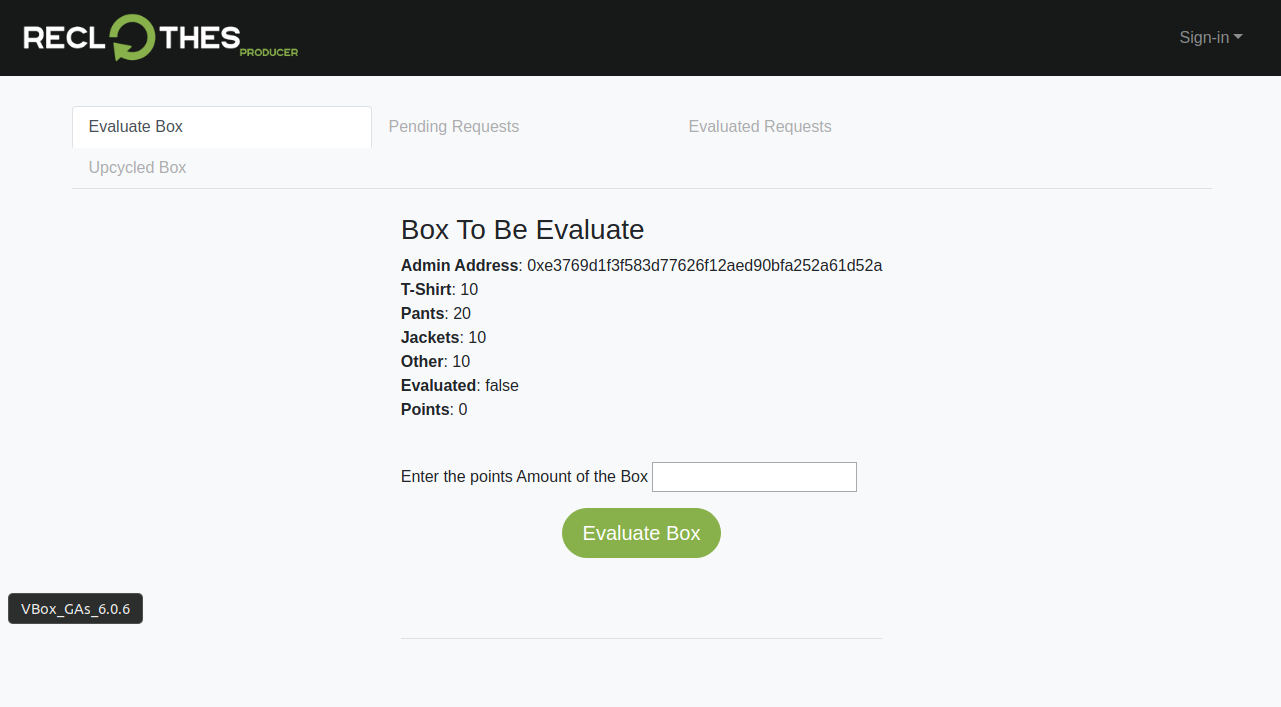
\includegraphics[totalheight=7cm]{img/test/usecase2/1-box-tobe-evaluate.png}
	\caption{Box to be evaluated}
	\label{fig:box-tobe-evaluate}
\end{figure}

\begin{figure}[h!]
	\centering
    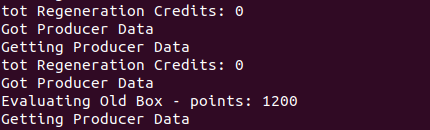
\includegraphics[totalheight=4cm]{img/test/usecase2/2-evaluation.png}
	\caption{Producer Evaluate old materials}
	\label{fig:evaluation-old-clothes}
\end{figure}

\begin{figure}[h!]
	\centering
    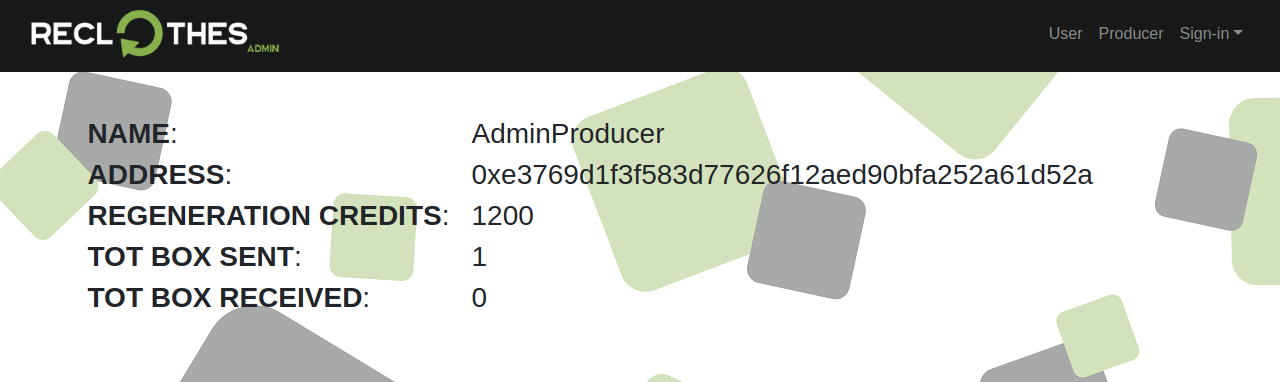
\includegraphics[totalheight=4cm]{img/test/usecase2/3-credits-received.png}
	\caption{Admin Info update}
	\label{fig:credits-received}
\end{figure}

\subsubsection{Purchase Upcycled Material}
 
Once the Admin sent box with old clothes and the evaluation process is archived, Admin has 
a Regeneration Credits amount to e spend to purchase upcycled clothes to send inside platform store.
In our test case we purchase a \textbf{Middle Box} going to spend 150 Regeneration Credits.
\\
The \textbf{Figure \ref{fig:buy-recycled-clothes}} show the output of purchase process and the 
Tot Regeneration Credits update after purchase box process is performed.
\\
The \textbf{Figure \ref{fig:producer-infos}} show the the update of Producer Informations,
the circulating Regeneration Credits amount is changed and the Tot Box New number too.

\begin{figure}[h!]
	\centering
    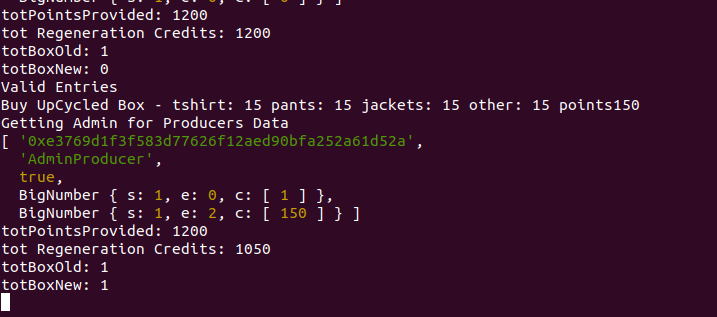
\includegraphics[totalheight=5cm]{img/test/usecase2/4-buy-recycled-clothes.png}
	\caption{Purchase Recycled Clothes}
	\label{fig:buy-recycled-clothes}
\end{figure}

\begin{figure}[h!]
	\centering
    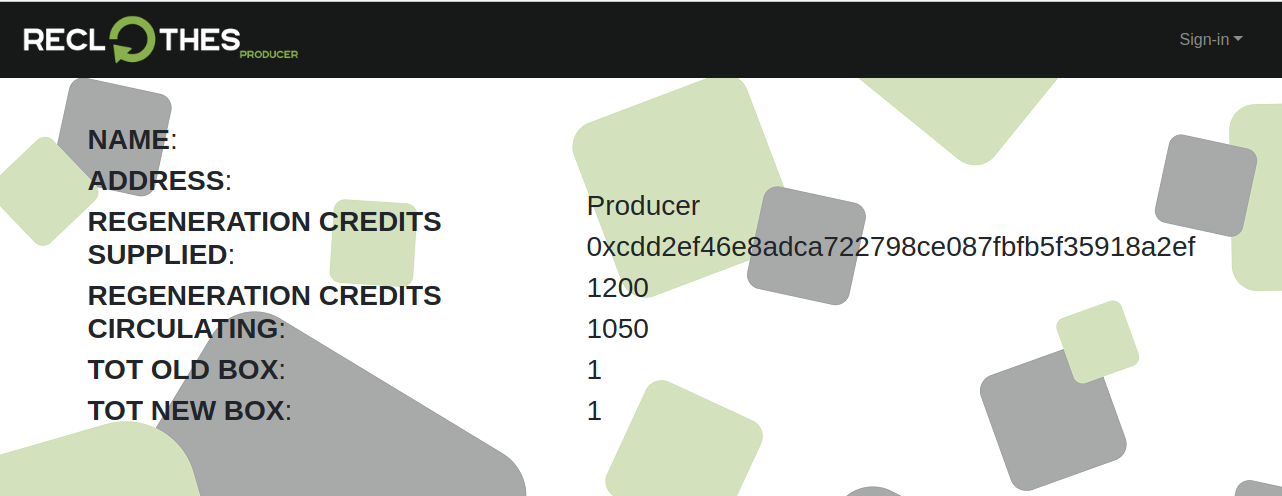
\includegraphics[totalheight=5cm]{img/test/usecase2/5-producer-info-update.png}
	\caption{Producer Infos Update}
	\label{fig:producer-infos}
\end{figure}